\newcommand{\NWtarget}[2]{#2}
\newcommand{\NWlink}[2]{#2}
\newcommand{\NWtxtMacroDefBy}{Fragment defined by}
\newcommand{\NWtxtMacroRefIn}{Fragment referenced in}
\newcommand{\NWtxtMacroNoRef}{Fragment never referenced}
\newcommand{\NWtxtDefBy}{Defined by}
\newcommand{\NWtxtRefIn}{Referenced in}
\newcommand{\NWtxtNoRef}{Not referenced}
\newcommand{\NWtxtFileDefBy}{File defined by}
\newcommand{\NWtxtIdentsUsed}{Uses:}
\newcommand{\NWtxtIdentsNotUsed}{Never used}
\newcommand{\NWtxtIdentsDefed}{Defines:}
\newcommand{\NWsep}{${\diamond}$}
\newcommand{\NWnotglobal}{(not defined globally)}
\newcommand{\NWuseHyperlinks}{}
\documentclass[12pt]{article}
\usepackage{graphicx}
\usepackage{amssymb}
\usepackage{listings}
\usepackage{amsmath}
\usepackage{graphicx}
\usepackage{float}
\usepackage[section]{placeins}
% Russian specicfic
% -------------------------
\usepackage[T2A]{fontenc}
\usepackage[utf8]{inputenc}
\usepackage[russian]{babel}
% -------------------------

\graphicspath{{./figs/}}

\begin{document}

\title{Общая связность сети. Критическое ребро.}

\author{
  Кирпа Вадим
  \and
  Махлярчук Андрей
  \and
  Утин Никита
  \and
  Березкин Аркадий
%  \and
%  Блинов Игорь
}

\maketitle
\thispagestyle{empty}
\newpage

\section{Постановка задачи:}

\paragraph{}
Для графа $G = (V, E, W)$ с множеством вершин $V$,
множеством ребер $W: E \rightarrow \mathbb{R}_+$
найти ребро $e^*$, такое, что при замене
$W(e^*) \rightarrow \gamma W(e^*)$ сумма сетевых 
расстояний между всеми узлами минимизируется
(при $\gamma < 1$) или максимизируется (при $\gamma > 1$).
Расчеты привести для графа Владивостока-2012.

\section{Алгоритм}

\paragraph{}
Для нахождения суммы сетевых расстояний в графе использовался
алгоритм Дейкстры\cite{dijkstra}.

\paragraph{}
Чтобы найти критическое ребро сумма сетевых расстояний считается
для всех подграфов $G_i$, где $W(e_i) \rightarrow \gamma W(e_i)$. Если сумма сетевых
ребер в текущем подграфе $G_i$ меньше (больше при $\gamma > 1$)
ранее найденой суммы, то это ребро сохраняется в качестве претендента
на критическое. В конце работы алгоритма мы получаем критическое ребро, 
сумму сетевых расстояний, соответствующую графу с обновленным весом критического ребра и новый вес данного ребра.

\section{Реализация} 
В начале выполнения программы происходит считывание графа из файла. 
Затем для каждой вершины запускаем алгоритм Дейкстры. В данной рализации можно было бы использовать 
алгоритм Флойда-Уоршелла, но было принято решение реализовать алгоритм Дейкстры, так как он легче поддается распараллеливанию.

\paragraph{}
Алгоритм реализован на языке C++. Основной процедурой является
алгоритм Дейкстры\cite{dijkstra}.


\subsection{Исходный код}
\paragragh{}
Приправа
\begin{flushleft} \small
\begin{minipage}{\linewidth}\label{scrap1}\raggedright\small
\NWtarget{nuweb11}{} \verb@"edge.h"@\nobreak\ {\footnotesize {11}}$\equiv$
\vspace{-1ex}
\begin{list}{}{} \item
\mbox{}\verb@@\\
\mbox{}\verb@#pragma once@\\
\mbox{}\verb@#include <atomic>@\\
\mbox{}\verb@#include <functional>@\\
\mbox{}\verb@@\\
\mbox{}\verb@class Edge {@\\
\mbox{}\verb@public:@\\
\mbox{}\verb@    Edge(const Edge& e) :left(e.left), right(e.right), weight(e.weight), travelCount(0) {} //todo check how to fix travelCount(e.travelCount)@\\
\mbox{}\verb@    Edge(int u, int v, double w) : left(u), right(v), weight(w), travelCount(0) {}@\\
\mbox{}\verb@    void IncTravelCount();@\\
\mbox{}\verb@    double GetTotalWeight();@\\
\mbox{}\verb@    const int GetLeft() const { return left; }@\\
\mbox{}\verb@    const int GetRight() const { return right; }@\\
\mbox{}\verb@    const double GetWeight() const { return weight; }@\\
\mbox{}\verb@    void SetWeight(double w) { weight = w; }@\\
\mbox{}\verb@private:@\\
\mbox{}\verb@    int left;@\\
\mbox{}\verb@    int right;@\\
\mbox{}\verb@    double weight;@\\
\mbox{}\verb@    std::atomic<int> travelCount;@\\
\mbox{}\verb@};@\\
\mbox{}\verb@@\\
\mbox{}\verb@struct EdgeHash {@\\
\mbox{}\verb@    unsigned int operator()(const Edge& e) const {@\\
\mbox{}\verb@        return std::hash<int>()(e.GetRight());@\\
\mbox{}\verb@    }@\\
\mbox{}\verb@};@\\
\mbox{}\verb@@\\
\mbox{}\verb@bool operator==(const Edge& e, const Edge& t);@\\
\mbox{}\verb@@{\NWsep}
\end{list}
\vspace{-1.5ex}
\footnotesize
\begin{list}{}{\setlength{\itemsep}{-\parsep}\setlength{\itemindent}{-\leftmargin}}

\item{}
\end{list}
\end{minipage}\vspace{4ex}
\end{flushleft}
\paragraph{Оцена вычислительной сложности алгоритма.}

На данном графе $G = (V, E, W)$, алгоритм Дейкстры имеет вычислительную  сложность $O(V \log V + E) $.
В нашем алгоритме на каждое изменение веса ребра, запускается алгоритм Дейкстры из каждой вершины. В результате получаем 
вычислительную сложность алгоритма $O((V \log V + E)VE)$

\paragraph{Оптимизации:}
Чтобы ускорить исполнение программы, из каждой
вершины алгоритм Дейкстры запускается в отдельном
потоке. Т.к. граф разрежен в памяти он хранится в
виде списка смежности.

\section{Результаты}

\subsection{Минимальный граф}

\paragraph{}

Рассмотрим простой пример работы алгоритма на графе с 6-ю вершинами и 5-ю ребрами
представленного на рис.~\ref{fig:min_graph_4} В данном случае мы будем минимизировать сумму сетевых расстояний и
примем $\gamma = 0.5$.

\begin{figure}[h]
    \centering
    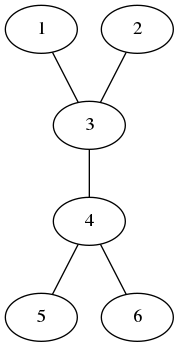
\includegraphics[scale=0.7]{min_graph_4.png}
    \caption{Минимальный граф с критическим ребром между 3-й и 4-й вершинами.}
    \label{fig:min_graph_4}
\end{figure}

Из каждой вершины исходного графа запустим алгоритм Дейкстры.
На каждом шаге работы алгоритма изменяем вес текущего ребра $W(e_i) \rightarrow \gamma W(e_i)$
Затем для данной итерации пересчитаем сумму сетевых расстояний, и, если она меньше текущей минимальной суммы,
то обновим минимум. Так в процессе работы алгоритма мы переберем все ребра и в качестве критического выберем 
ребро с соответствующей минимальной суммой сетевых расстояний. 
На каждой итерации работы алгоритма Дейкстры получим сумму сетевых расстояний для исходного графа:

\begin{gather}
1 : 1 + 5 + 6 + 6 + 2 \\
2 : 1 + 5 + 6 + 6 + 2 \\
3 : 1 + 1 + 4 + 5 + 5 \\
4 : 1 + 1 + 4 + 5 + 5 \\
5 : 1 + 5 + 6 + 6 + 2 \\
6 : 1 + 5 + 6 + 6 + 2
\end{gather}

Сумма сетевых расстояний в исходном графе $S = 112$. 

\begin{figure}[h]
    \centering
    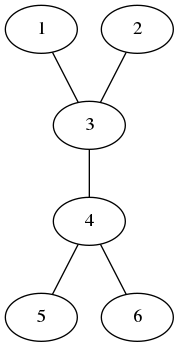
\includegraphics[scale=0.7]{min_graph_2.png}
    \caption{Если уменьшить вес ребра между 3-й и 4-й вершинами сумма сетевых расстояний минимизируется}
    \label{fig:min_graph_2}
\end{figure}

В данном граффе критическим является ребро между
3й и 4й вершинами и умножение его веса на
$\gamma < 1$ приводит к минимизации суммы сетевых расстояний.
При $\gamma = 0.5$ алгоритм меняет вес критического ребра на $0.5 \cdot w_i$ (рис.~\ref{fig:min_graph_2}).
Для обновленного графа, в котором мы заменили вес критического ребра на 2 получим сумму сетевых расстояний:

\begin{gather}
1 : 1 + 3 + 4 + 4 + 2 \\
2 : 1 + 3 + 4 + 4 + 2 \\
3 : 1 + 1 + 2 + 3 + 3 \\
4 : 1 + 1 + 2 + 3 + 3 \\
5 : 1 + 3 + 4 + 4 + 2 \\
6 : 1 + 3 + 4 + 4 + 2
\end{gather}

В таком случае сумма сетевых расстояний для обновленного графа будет равнятся $S^* = 76$.

\paragraph{При $\gamma = 2 > 1$.}
Алгоритм меняет вес критического ребра на $2 \cdot w_i = 8$ (рис.~\ref{fig:min_graph_8}).

\begin{figure}[h]
    \centering
    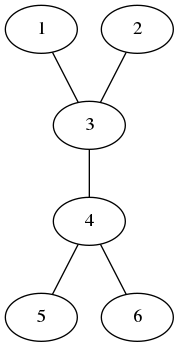
\includegraphics[scale=0.7]{min_graph_8.png}
    \caption{Если увеличить вес ребра между 3-й и 4-й вершинами сумма сетевых расстояний максимизируется}
    \label{fig:min_graph_8}
\end{figure}

В обновленном графе, с весом критического ребра = 8 мы получим следующую
сумму сетевых расстояний:

\begin{gather}
1 : 1 + 9 + 10 + 10 + 2 \\
2 : 1 + 9 + 10 + 10 + 2 \\
3 : 1 + 1 + 8  + 9  + 9 \\
4 : 1 + 1 + 8  + 9  + 9 \\
5 : 1 + 9 + 10 + 10 + 2 \\
6 : 1 + 9 + 10 + 10 + 2
\end{gather}

Что дает сумму сетевых расстояний равную $S^* = 184$

\subsection{Граф малого размера (20 вершин)}

\paragraph{}
При запуске на графе малого размера (рис~\ref{fig:small}) 
алгоритм корректно определил критическое ребро.
Этому ребру был намеренно предан большой вес для удобства тестирования.
При $k = 0.5$ и при $k = 1.5$ алгоритм определял одно
и то же ребро между 19-й и 20-й вершинами (отмечено красным),
однако изменение веса этого ребра приводило к разным итоговым
суммам сетевых расстояний, а именно к $12542$ и $14264$ соотвественно.

\begin{figure}[h]
    \centering
    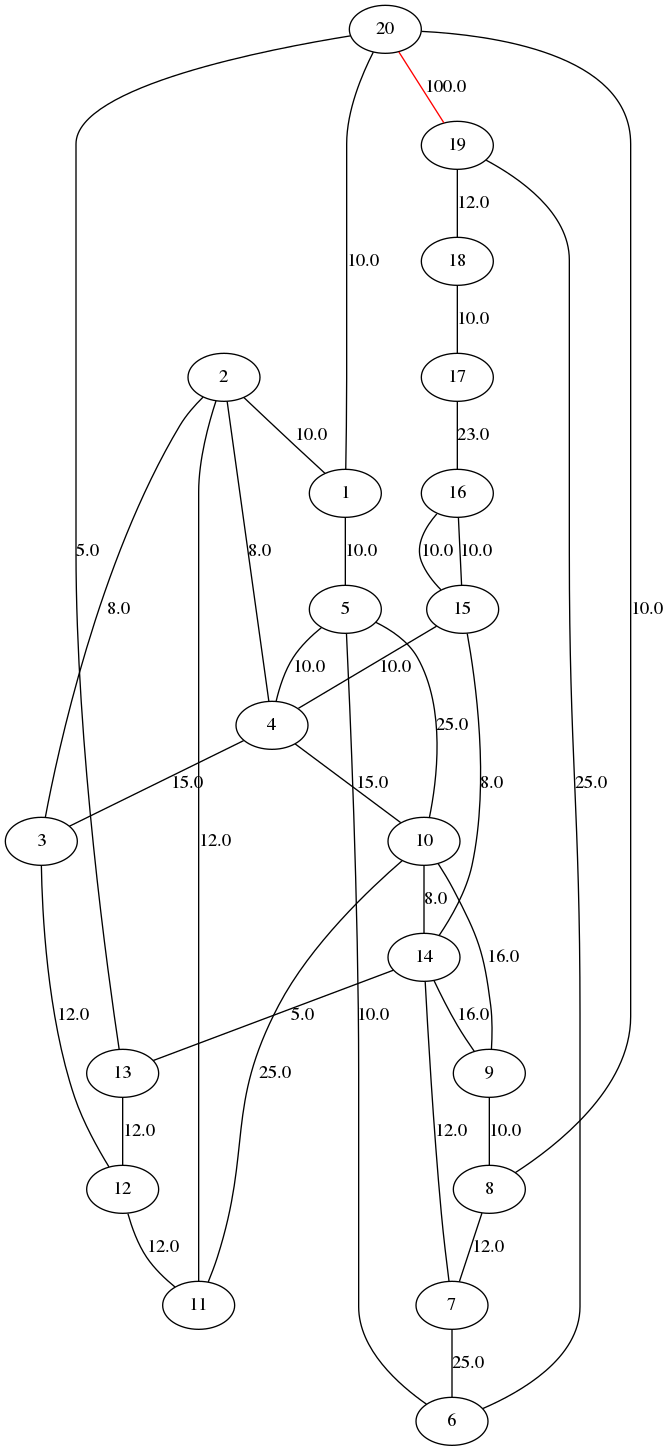
\includegraphics[scale=0.3]{small.png}
    \caption{Малый граф с 20-ю вершинами. Критическое ребро отмечено красным.}
    \label{fig:small}
\end{figure}

\subsection{Граф среднего размера (~1500 вершин)}

\paragraph{}
В качестве графа среднего размера был взят сокращеное представление 
транспортной сети города Владивостока на 2009-й годi (рис.~\ref{vlad_2009}). 
В данном представлении 1542 вершины и 1653 ребра.

\begin{figure}[h]
    \centering
    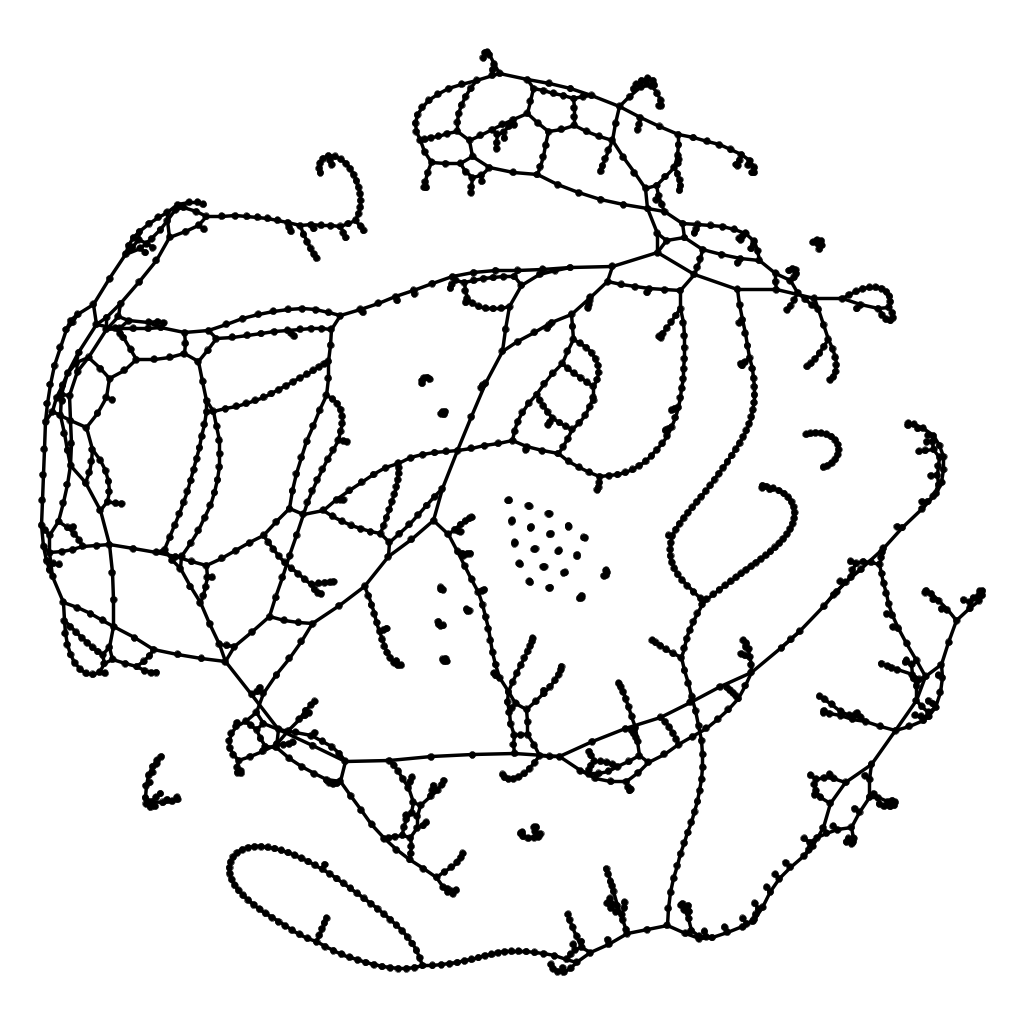
\includegraphics[scale=0.3]{vlad_2009.png}
    \caption{Сокращенная транспортная сеть города Владивостока на 2009-й год.}
    \label{fig:vlad_2009}
\end{figure}

\paragraph{}
Алгоритм был запущен с значениями $k = 0.5$ и $k = 1.5$ и определил различные
критические ребра. Ребро между

% New distances: 2.60341e+10. With edge between 175 and 176. Weight: 1008.3; k = 0.5
% New distances: 2.67274e+10. With edge between 175 and 176. Weight: 1008.3; k = 1.5

\begin{figure}[h]
    \centering
    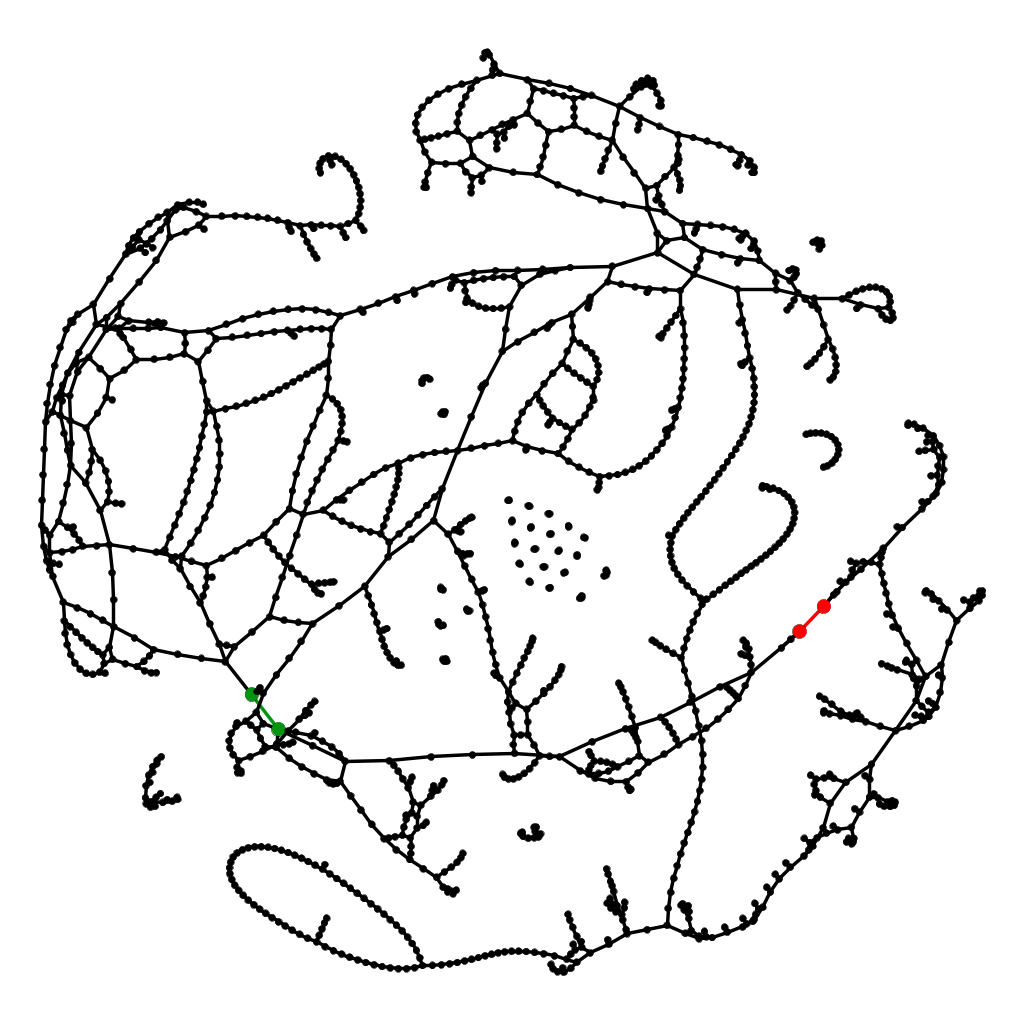
\includegraphics[scale=0.3]{vlad_2009_min_max.png}
    \caption{Сокращенная транспортная сеть города Владивостока на 2009-й год.}
    \label{fig:vlad_2009_min_max}
\end{figure}

\section{Заключение}
Окончательное и обжалованию не подлежит

\newpage

\begin{thebibliography}{9}
\bibitem{dijkstra}
Dijkstra E. W. \textit{A note on two problems in connexion with graphs} //
\textit{Numer. Math} — Springer Science+Business Media, 1959.
— Vol. 1, Iss. 1. — P. 269–271.
\end{thebibliography}

\end{document}
